

\section{Efficiently calibrating a model}

We now turn to the question of how to produce models that we can \emph{verify} are calibrated.
We describe the variance-reduced calibrator (Figure~\ref{fig:variance_reduced_illustration}), and prove bounds on its sample complexity.
In particular, assuming the function familty $\mathcal{G}$ is well suited to recalibrate the data, we require $O(\frac{1}{\epsilon^2})$ samples to achieve calibration error $\epsilon$, while histogram binning requires $O(\frac{B}{\epsilon^2})$ samples.
Moreover, unlike methods such as Platt scaling and temperature scaling, we can then check if our model is calibrated (see Section~\ref{sec:verifying_calibration}).
If the model is not calibrated we can, for example, try different families $\mathcal{G}$ or collect more data and use histogram binning.

% Models obtained by performing empirical risk minimization on a training set tend to be uncalibrated. Typically, we apply recalibration methods that take the output of an uncalibrated model, and transform it into a calibrated probability. These methods require additional held-out \emph{recalibration data}. 

% \textbf{Recalibration framework:} We now turn to the question of how to produce models that \emph{we can verify are calibrated}. Models obtained by performing empirical risk minimization on a training set tend to be uncalibrated. Typically, we apply post-processing methods that take the output of an uncalibrated model, and transform it into a calibrated probability. These methods require an additional held-out \emph{calibration set}.

% \textbf{Histogram binning:} One common method for recalibration is histogram binning. The outputs of the model (on the calibration set) are divided into disjoint intervals $I_1, ..., I_B$. At test time, if the model's output falls into interval $I_j$, we output $s_j$ where $s_j$ is the proportion of examples in $I_j$ that were positive in the calibration set. \ak{Either make more clear and/or refer to another paper} The advantage of histogram binning is that in the limit of infinite data it will be perfectly calibrated. However, achieving $\ell_2$ calibration error $\epsilon$ with $B$ bins can require up to $O(\frac{B}{\epsilon^2})$ samples.

% \textbf{Variance-reduced calibration:} We introduce variance-reduced calibration, a more sample-efficient way to calibrate, and analyze the sample complexity of our methods. Like in Platt scaling, we first fit a function from a function family $\mathcal{F}$ to the data. Then, we identify a suitable binning scheme, and discretize the outputs of our model. Restricting to the function family $\mathcal{F}$ introduces some bias -- if $\mathcal{F}$ is poorly chosen, then even in the limit of infinite data we may not be able to calibrate. However, if $\mathcal{F}$ is well-chosen, we will be able to calibrate with far fewer samples.

% \textbf{Calibration verifiable:} Moreover, unlike methods such as Platt scaling and temperature scaling, we can then check if our model is calibrated using techniques described in the previous section. If the model is not calibrated we can, for example, try different families $\mathcal{F}$ or collect more data and use histogram binning.

% The highlights of our analysis include:
% \begin{enumerate}
% \item We show that discretizing approaches like Platt scaling, isotonic regression, or temperature scaling, requires very few samples (Theorem~\ref{thm:empirical-binning}). Surprisingly, the number of samples required only has logarithmic dependencies on $B$.
% \item We show that we only need $n = O(B\log{B})$ samples to select a lower-balanced binning scheme (Theorem~\ref{thm:well-ba-binning}). Standard results on concentration of functions like Dvoretzky–Kiefer–Wolfowitz or VC dimension give us $n = O(B^2\log{B})$.
% \item We show that discretizing the outputs of our model has little impact on model quality, measured in terms of the Brier score (also known as the mean-squared error) (Theorem~\ref{thm:sharpness-bound}).
% \end{enumerate}
% We believe we are the first to give a formal framework for the statistics of calibration, which can guide future work in this area.

% There are two general approaches to recalibration. The first is histogram binning, where we output the average label value observed in each bin. The advantage of histogram binning is that in the limit of infinite data it will be perfectly calibrated. However, to achieve $\ell_2$ calibration error $\epsilon$ with $B$ bins it requires $O(\frac{B}{\epsilon^2})$ samples.\footnote{This analysis is standard, so we omit it from our paper.} The second is to fit a function, like a sigmoid function in the case of Platt scaling, and then discretize the model outputs. If this approach can calibrate to within error $\epsilon$,\footnote{Depending on the function family, this approach may, or may not, ever achieve good calibration.} it requires only $O(\frac{1}{\epsilon^2})$ samples to do so. In particular, estimating the calibration error ($O(\frac{B}{\epsilon^2})$ with prior approaches, and $O(\frac{\sqrt{B}}{\epsilon^2})$ with our estimator) is then the bottleneck. This is the focus of our analysis which concludes with Theorem~\ref{thm:final-calib} and Theorem~\ref{thm:sharpness-bound}. In practice, we would try multiple re-calibration approaches, estimate the calibration error using our estimator, and choose the best one.

\subsection{Variance-reduced calibration algorithm}

Suppose we are given a trained model $f: \mathcal{X} \to \mathcal{Z}$ that we wish to calibrate. As before, $X \in \mathcal{X}$ and $Y \in \{0, 1\}$ are random variables denoting the input and label, given by an unknown joint distribution $P(X, Y)$. We wish to learn $\hat{g_{\mathcal{B}}} : \mathcal{Z} \to [0, 1]$ such that $\hat{g_{\mathcal{B}}} \circ f$ is well-calibrated. Let $Z = f(X)$.

Let $\mathcal{G}$ be a family of functions from $\mathcal{Z} \to [0, 1]$, and $B$ be the number of outputs for the final model. Like other calibration methods, we require additional i.i.d. calibration data $T = \{ z_i, y_i \}_{i=1}^n$ where $z_i, y_i \sim P(Z, Y)$ for all $i$. We split $T$ into 3 sets: $T_1$, $T_2$, $T_3$. We begin with a definition.

\begin{definition}[Binning schemes]
A binning scheme $\mathcal{B}$ of size $B$ partitions $[0, 1]$ into $B$ disjoint intervals or bins, defined by bin boundaries $0 = b_0 < b_1 < ... < b_B = 1$. For $1 \leq j \leq B$, the $j$-th bin is the interval $I_j$ where $I_1 = [b_0, b_1]$ and $I_j = (b_{j-1}, b_j]$ for $j > 1$. Given an input $x \in [0, 1]$ we might want to know what bin it falls in -- if $x \in I_j$ let $\beta(x) = j$.
\end{definition}

Now we describe the variance-reduced calibration algorithm, illustrated in Figure~\ref{fig:variance_reduced_illustration}.

% \footnote{The optimal way to select $T$ depends on $F$, and our analysis in the next subsection.}

\textbf{Step 1 (Function fitting):} The first step is to select $g = \argmax_{g \in G} \sum_{(z, y) \in T_1} (y - g(z))^2$.

\textbf{Step 2 (Bin construction):} The second step is to identify a suitable binning scheme. We choose the bins so that an equal number of $g(z_i)$ land in each bin. Formally, given interval $I$ and dataset $T$, let $N(I, T) = \frac{1}{|T|}\sum_{(z, y) \in T} \mathbb{I}(g(z) \in I)$. We choose bins such that $N(I_j, T_2) = \frac{1}{B}$ for all $1 \leq j \leq B$. 

\textbf{Step 3 (Discretization):} The third step is to discretize $g$, by outputting the average $g$ value in each bin. Let $\mu(S) = \frac{1}{|S|} \sum_{s \in S} s$ denote the mean of a set of values.
% Let $R_j(T) = \{ g(z_i) \; | \; g(z_i) \in I_j \wedge (z_i, y_i) \in T \}$.
% Let $\hat{\mu}[j] = \mu(R_j(T_3))$ be the mean of the $g(z_i)$ values in the $j$-th bin.
Let $\hat{\mu}[j] = \mu(\{ g(z_i) \; | \; g(z_i) \in I_j \wedge (z_i, y_i) \in T_3 \})$ be the mean of the $g(z_i)$ values that landed in the $j$-th bin.
Then we set $\hat{g_{\mathcal{B}}}(z) = \hat{\mu}[\beta(g(z))]$ -- that is we simply output the mean value in the bin that $g(z)$ falls in.

\subsection{Analysis}

% \begin{definition}
% Let $f^* : \mathcal{Z} \to [0, 1]$ be the sharpest recalibrator, defined as $f^*(z) = \mathbb{E}_P[Y | Z = z]$. 
% \end{definition}

% \begin{definition}
% We say a family of functions $\mathcal{F}$ from $\mathcal{Z} \to [0, 1]$ is $\epsilon$-specified if there exists $f \in \mathcal{F}$ s.t. $||f - f^*||_2 \leq \epsilon$. If $\epsilon = 0$, then we say $\mathcal{F}$ is well-specified.
% \end{definition}

Our analysis requires some assumptions on the function family $\mathcal{G}$:
\begin{enumerate}
\item (Finite bounded parameters). Let $\mathcal{G} = \{ g_{\theta} : \mathcal{Z} \to [0, 1] \; | \; \theta \in \mathbb{R}^{d'} \wedge ||\theta||_{\infty} \leq B \}$
\item (Injective). For all $g_{\theta} \in \mathcal{G}$ we assume $g_{\theta}$ is injective.
\item (Lipschitz). Suppose that for all $z$, $|g_{\theta_1}(z) - g_{\theta_2}(z)| \leq L|\theta_1 - \theta_2|_2$.
\end{enumerate}

Assumptions (1) and (3) are standard in statistical learning theory. Assumption (2) holds for methods like Platt scaling, Beta calibration~\cite{kull2017sigmoids}, and vector scaling, but we hope future work relaxes this.

% We assume the function family $\mathcal{F}$ is chosen such that given infinite data, minimizing the mean-squared error loss leads to a well-calibrated solution.

% \begin{proposition}[Error from empirical risk minimization]
% \label{thm:mse-convergence}
%  There exists a constant $c$ such that the following holds. For $\theta \in  \mathbb{R}^{d'}$ let $f_{\theta} : \mathcal{Z} \to [0, 1]$ be injective. Suppose that for all $z$, $|f(z; \theta_1) - f(z; \theta_2)| \leq L|\theta_1 - \theta_2|_2$. Let $\mathcal{F} = \{ f_{\theta} \; | \; \theta \in \mathbb{R}^{d'} \wedge ||\theta||_{\infty} \leq B \}$, and let $f^* = \argmin_{f \in \mathcal{F}}{E[(f(Z) - Y)^2]}$. Then with probability $\geq 1 - \delta$ (over the samples) $\ell_2\mbox{-CE}(f) \leq \ell_2\mbox{-CE}(f^*) + \frac{cLd' \log{B/\delta}}{\sqrt{n}}$. 
% \end{proposition}

% We chose a binning scheme such that each bin had an equal proportion of points in the calibration set. We show that this property approximately holds in the population as well.

% \begin{definition}[Well-balanced binning]
% Given a binning scheme $\mathcal{B}$ of size $B$, and $\alpha \leq 1$. We say $\mathcal{B}$ is $\alpha$-well-balanced if for all $j$,
% \[ \frac{1}{\alpha B} \leq P(Z \in I_j) \leq \frac{\alpha}{B}\]
% \end{definition}

% \begin{theorem}[Population well-balanced]
% \label{thm:well-ba-binning}
% If we use $O(B \log{B})$ samples in step 2 of our algorithm, the binning scheme we select will be 2-well-balanced.
% \end{theorem}

% Next, we show that if we had infinite data, discretizing $f$ can only decrease its calibration error.

% \begin{definition}
% Given $f : \mathcal{Z} \to [0, 1]$, and a binning scheme $\mathcal{B}$, let $f_{\mathcal{B}}$ denote the discretized version of $f$ where we take the average value of $f$ in each bin. Formally, $f_{\mathcal{B}}(z) = \mathbb{E}[f(Z) | f(Z) \in I_{\beta(f(z))}]$. 
% \end{definition}

% \begin{lemma}[Binning improves calibration]
% \label{lem:inf-binning}
% [Binning improves calibration] Given $f : \mathcal{Z} \to [0, 1]$ and binning scheme $\mathcal{B}$, $\ell_2\mbox{-CE}(f_{\mathcal{B}}) \leq \ell_2\mbox{-CE}(f)$.
% \end{lemma}

% In step 3 of our algorithm, we use finitely many samples to discretize the outputs of $f$, to get an approximation $\hat{f_{\mathcal{B}}}$. We show that $f_{\mathcal{B}}$ -- the discretized version of $f$ when we have infinite data -- and $\hat{f_{\mathcal{B}}}$ are close in both $\ell_1$ and $\ell_2$ distance.

% \begin{definition} [$\ell_1, \ell_2$ distance]
% Given $f, g : \mathcal{Z} \to [0, 1]$, we define $|f - g|_2^2 = \mathbb{E}[(f(Z) - g(Z))^2]$, $||f- g||_2 = \sqrt{|f - g|_2^2}$, and $|f- g|_1 = \mathbb{E}[\lvert f(Z) - g(Z) \rvert]$.
% \end{definition}

% \begin{theorem}[Error from empirical binning]
% \label{thm:empirical-binning}
% There exist constants $c_B, c_1, c_2$ such that the following is true. Given $f : \mathcal{Z} \to [0, 1]$, binning set $T = \{(z_i, y_i)\}_{i=1}^n$ and a 2-well-balanced binning scheme $\mathcal{B}$ of size $B$. Given $0 < \delta < 0.5$, suppose that $n \geq c_B B\log{\frac{B}{\delta}}$. Then with probability at least $1 - \delta$,  $|\hat{f_{\mathcal{B}}} - f_{\mathcal{B}}|_2 \leq \frac{c_2}{\sqrt{n}}\sqrt{\log{\frac{B}{\delta}}}$ and $|\hat{f_{\mathcal{B}}} - f_{\mathcal{B}}|_1 \leq \frac{c_1}{\sqrt{nB}}\sqrt{\log{\frac{B}{\delta}}}$
% \end{theorem}

% We use this to bound the calibration error of $\hat{f_{\mathcal{B}}}$ with a simple lemma.

% \begin{lemma}
% For all $f, g : Z \to [0, 1]$, $\ell_2\mbox{-CE}(f) \leq \ell_2\mbox{-CE}(g) + |f - g|_2$.
% \end{lemma}

% Putting these together, we get our final bound on calibration error.

We chose a binning scheme such that each bin had an equal proportion of points in the calibration set. Crucially, we will show that this property approximately holds in the population as well.

\begin{definition}[Well-balanced binning]
Given a binning scheme $\mathcal{B}$ of size $B$, and $\alpha \leq 1$. We say $\mathcal{B}$ is $\alpha$-well-balanced if for all $j$,
\[ \frac{1}{\alpha B} \leq P(Z \in I_j) \leq \frac{\alpha}{B}\]
\end{definition}

We now present the main theorem, which shows that if $\mathcal{G}$ contains $g^*$ with low calibration error, then our method will quickly find $\hat{g}_{\mathcal{B}}$ with low calibration error. Further, the binning scheme $\mathcal{B}$ we produce will be 2-well-balanced, which will allow us to measure the calibration error efficiently as described in the next section (Theorem~\ref{thm:final-ours}).

\begin{theorem}[Calibration bound]
\label{thm:final-calib}
Suppose that $\min_{g \in \mathcal{G}}\ell_2^2\mbox{-CE}(g) \leq \epsilon^2$.
Ignoring $\log$ factors, with $n = O(B + \frac{L^2 (d')^2}{\epsilon^2})$ samples the variance-reduced calibration algorithm produces a 2-well-balanced binning scheme and $\hat{g}_{\mathcal{B}}$ with $\ell_2^2\mbox{-CE}(\hat{f}_{\mathcal{B}}) \leq 2 \epsilon^2$. Note that $d' = 1$ for Platt scaling.
\end{theorem}

We give a proof of this result in the Appendix. The key steps are to (1) show that by optimizing the mean-squared error we will find a $g \in \mathcal{G}$ with low calibration error, (2) the binning scheme we constructed is 2-well-balanced (on the population), and finally (3) the number of samples required to empirically discretize $g$ to get $\hat{g}_{\mathcal{B}}$ only has logarithmic dependencies on the number of outputs $B$.

We also show that if we use lots of bins, discretization has little impact on model quality as measured by the Brier score (the mean-squared error):

\begin{theorem}[Sharpness bound]
\label{thm:sharpness-bound}
If $\mathcal{B}$ is a 2-well-balanced binning scheme of size $B$ and $B \leq O(n\log{n})$, then with high probability $\mbox{MSE}(\hat{g}_{\mathcal{B}}) \leq \mbox{MSE}(g) + O(\frac{1}{B})$.
\end{theorem}

\subsection{Experiments}

We ran experiments on CIFAR-10 and ImageNet to compare our variance-reduced calibrator with histogram binning. The model's objective was to output a confidence score associated with each class and we evaluated calibration using the marginal calibration error (Definition~\ref{dfn:marginal-ce}). Our results show that in the low-data regime, for example when we use $\leq 1000$ data points to recalibrate, our method produces models with much lower calibration error. 

We describe our experimental protocol for CIFAR-10.
The CIFAR-10 validation set has 10,000 data points. We sampled, with replacement, a recalibration set of 1,000 points. We ran our variance-reduced calibrator (we fit a sigmoid in the function fitting step) and histogram binning and measured the marginal calibration error on the entire set of 10K points.
% \footnote{This is equivalent to using the empirical distribution on the 10K validation points as the true data distribution, and comparing how these methods perform. We do this since we cannot measure the ground truth calibration error.}
We repeated this entire procedure 100 times and computed mean and 90\% confidence intervals, and we repeated this varying the number of bins $B$, showing the results in Figure~\ref{fig:marginal_calibrator_comparison_cifar}.

Using more bins allows a model to produce more fine-grained predictions, which can be measured by the mean-squared error. Figure~\ref{fig:cifar_calibrator_cmp_mse_ce} is a scatter plot of the mean-squared error and $\ell_2^2$ calibration error for each of these runs. In the Appendix, we show results for top-label calibration, for ImageNet, when we use more than 1,000 data points, and if we use an alternative binning scheme, the one in~\cite{guo2017calibration} -- this binning scheme does not have the same theoretical guarantees and performs worse in practice.

\begin{figure}
  \centering
  \centering
     \begin{subfigure}[b]{0.55\textwidth}
         \centering
         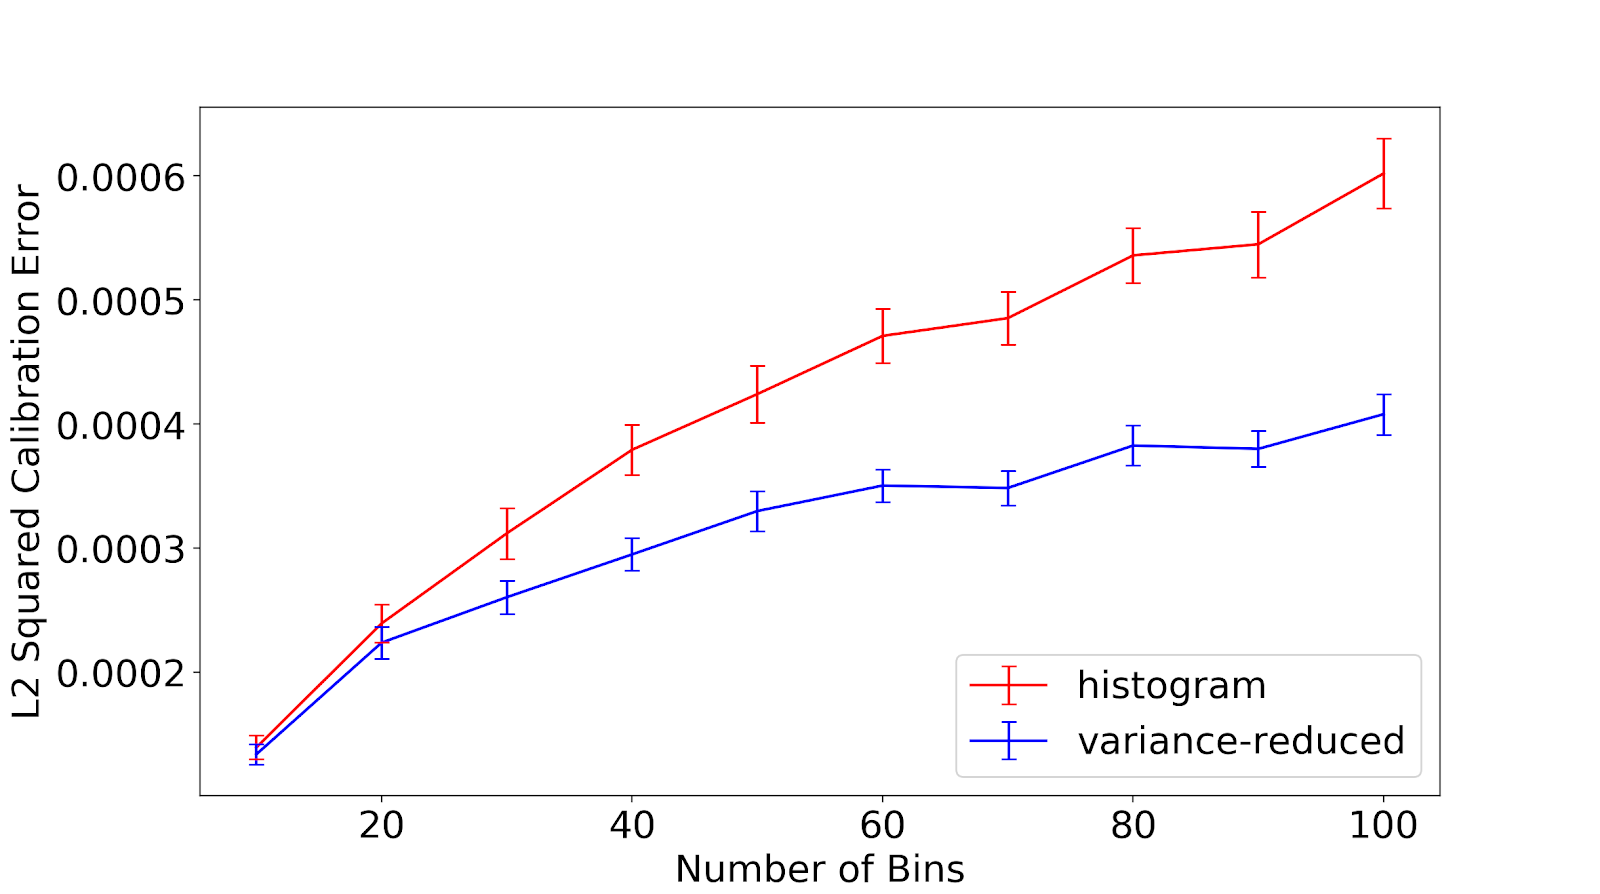
\includegraphics[width=\textwidth]{marginal_cifar_hist_vs_ours_bins.png}
         \caption{$\ell_2^2$ calibration error vs $B$.}
         \label{fig:marginal_calibrator_comparison_cifar}
     \end{subfigure}
     \hfill
     \begin{subfigure}[b]{0.4\textwidth}
         \centering
         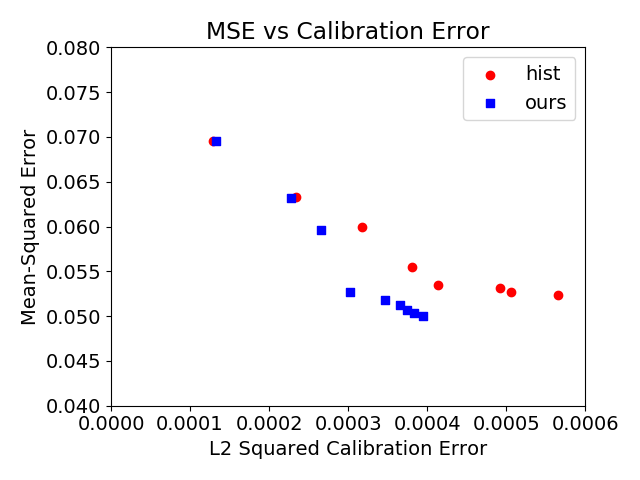
\includegraphics[width=\textwidth]{mse_vs_ce_calibrators_cifar.png}
         \caption{MSE vs $\ell_2^2$ calibration error.}
         \label{fig:cifar_calibrator_cmp_mse_ce}
     \end{subfigure}
  \caption{
  (\textbf{Left}) Recalibrating using 1,000 data points on CIFAR-10, our variance-reduced calibrator achieves lower $\ell_2^2$ calibration error than histogram binning, especially when the number of bins $B$ is large.
  (\textbf{Right}) For a fixed calibration error, our variance-reduced calibrator allows us to use more bins. This results in models with more predictive power which can be measured by the mean-squared error.
  }
  \label{fig:nan2}
\end{figure}

